\input{slide_style.tex}
\title{Workshop introduction}
\setbeamertemplate{headline}{}
\begin{document}
\begin{frame}[plain]
\centering
{\Huge\textcolor{NordBlue}{HOTPOT Workshop}\par}
\vspace{12pt}
{\large A \textbf{H}ands-\textbf{O}n \textbf{T}utorial for \textbf{P}hysical\par
Design with \textbf{O}pen-Source \textbf{T}ools\par}
\vspace{18pt}
{\large Monday - Wednesday\par}
\vspace{5pt}
{\large 21 - 23 September 2026\par}
\end{frame}

\begin{frame}{The plan}
\centering
\includegraphics[width=\textwidth,height=.83\textheight,keepaspectratio]{images/workshop-schedule.pdf}
\note{Day 1 introduces cell libraries, file formats, OpenROAD and floorplanning. Day 2 covers global placement, detailed placement and clock-tree synthesis. Day 3 covers global routing, detailed routing, finishing and getting chips made. The new first block groups Cell library, Design files and Flow script. All eight blocks have identical widths, heights and gaps; the Day 1 heading has no extra explanatory text. The seven stage views show the same Nangate45 GCD design from this repository's saved checkpoints. Floorplan rows and placement cell boundaries are drawn as vector abstractions from the exact OpenDB geometry; internal pin patterns are omitted at thumbnail scale. CTS is an original vector redraw of actual placed cells and clock terminal coordinates: grey cells, purple flip-flops, green clock buffers, blue connectivity fly-lines. These lines are not routed clock metal. Global routing shows the actual route-guide segments. Detailed routing is rendered from the final routed OpenDB with filler instances hidden. Finishing is a native KLayout image of design.gds, merged from gcd\_final.def and the Nangate45 standard-cell GDS using the upstream OpenROAD-flow-scripts def2stream.py. The existing asiclab Nangate45 .lyp supplies the colors and drawing order. No empty or orphan GDS cells remain. All 671 filler cells are present, matching the DEF; they have well/implant and rail shapes but no transistor gates. These views share final route geometry because no separate pre-filler checkpoint was saved. Rebuild using make stages finishing overview.}
\end{frame}

\begin{frame}{Workshop logistics}
\begin{columns}[c,onlytextwidth]
\begin{column}{.60\textwidth}
\fontsize{9}{11}\selectfont
\begin{itemize}\setlength{\itemsep}{10pt}
\item Schedule
  \begin{itemize}\setlength{\itemsep}{4pt}
  \item Monday 21 September: 10:00 - 18:00
  \item Tuesday 22 September: 10:00 - 18:00
  \item Wednesday 23 September: 10:00 - 14:00
  \end{itemize}
\item All talks and exercises in this room
\item Complimentary lunch each day at \textasciitilde13:00
\item We'll have an unofficial dinner tonight
\end{itemize}
\end{column}
\begin{column}{.36\textwidth}
\centering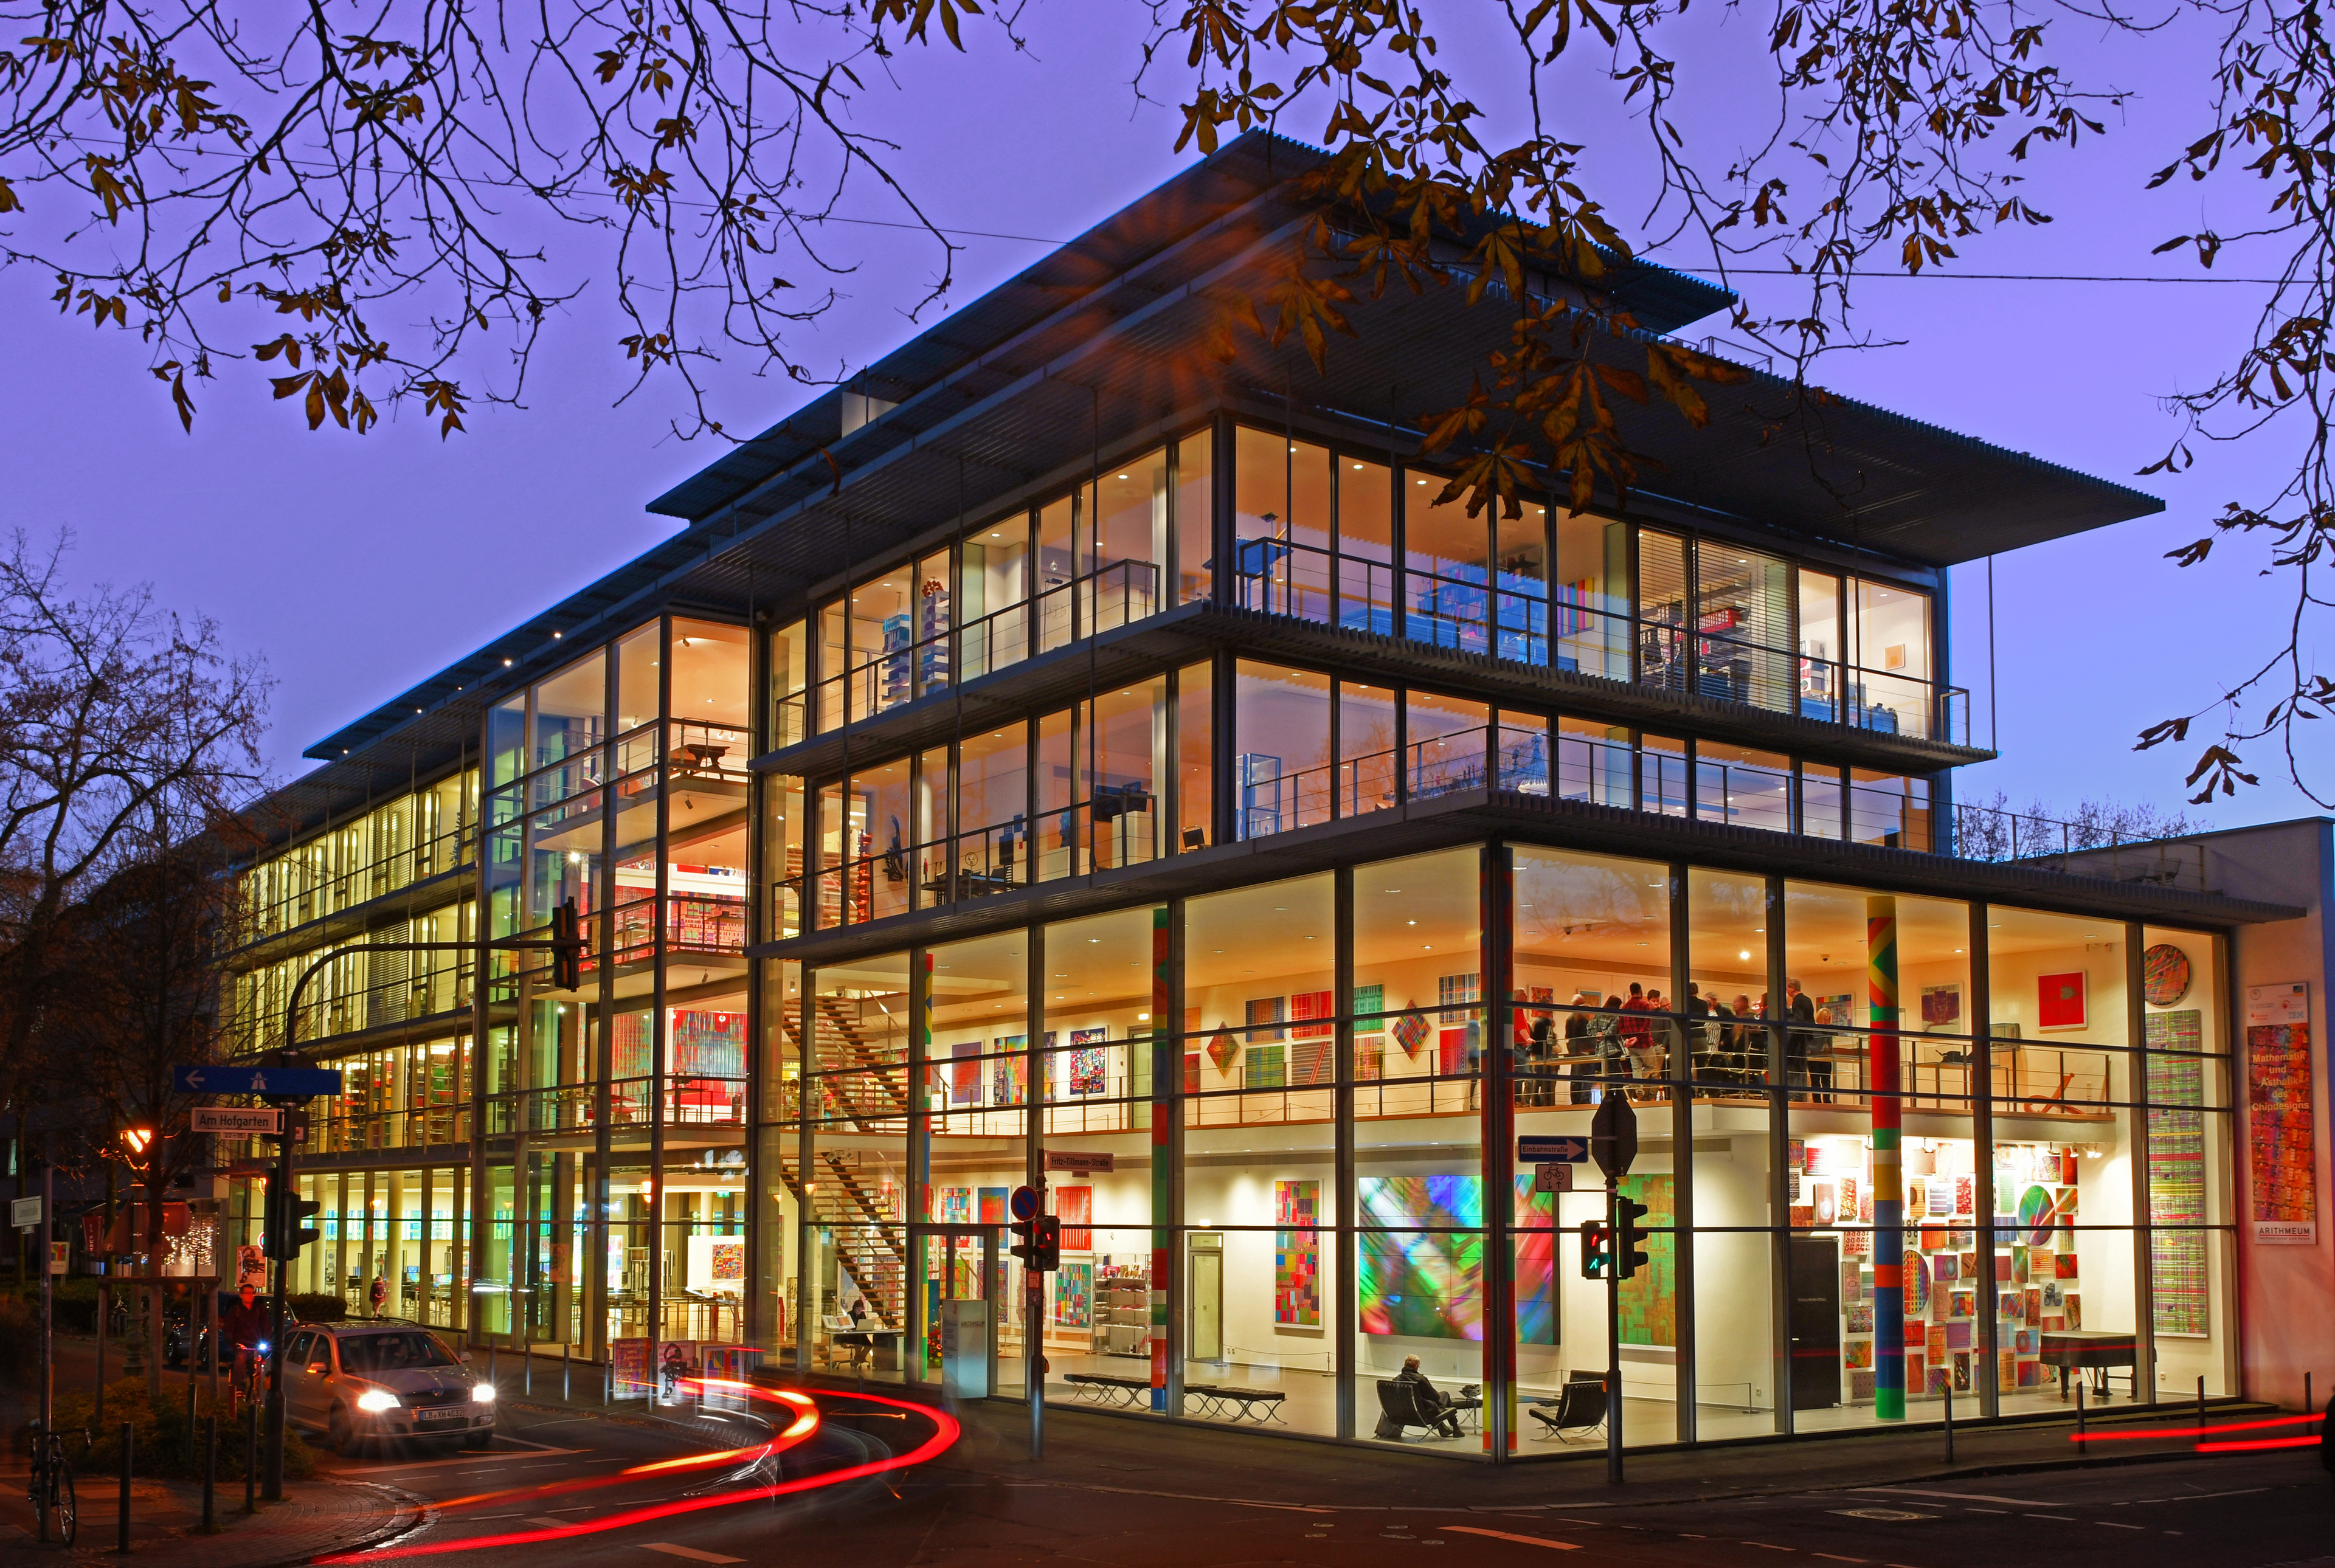
\includegraphics[width=\linewidth]{images/arithmeum-house.jpg}
\end{column}
\end{columns}
\note{Workshop dates: 21--23 September 2026. Monday: cell design, design file formats and floorplanning. Tuesday: placement and timing. Wednesday: global and detailed routing, finishing and getting chips made. The user supplied the schedule and meal information. The visible logistics are limited to dates, times, the conference room, lunch and dinner. “Today” is spoken from the Monday workshop presentation date. Building photograph supplied by the user: https://www.arithmeum.uni-bonn.de/fileadmin/user_upload/Arithmeum-Hausfoto.jpg . Sources are retained in notes only, as requested for the intro deck. Photo retained without cropping.}
\end{frame}
\end{document}
